%%%%%%%%%%%%%%%%%%%%%%%%%%%%%%%%%%%%%%%%%%%%%%%%%%%%%%%%%%%%%%%%%%%%%%
% LaTeX Example: Project Report
%
% Source: http://www.howtotex.com
%
% Feel free to distribute this example, but please keep the referral
% to howtotex.com
% Date: March 2011 
% 
%%%%%%%%%%%%%%%%%%%%%%%%%%%%%%%%%%%%%%%%%%%%%%%%%%%%%%%%%%%%%%%%%%%%%%
% How to use writeLaTeX: 
%
% You edit the source code here on the left, and the preview on the
% right shows you the result within a few seconds.
%
% Bookmark this page and share the URL with your co-authors. They can
% edit at the same time!
%
% You can upload figures, bibliographies, custom classes and
% styles using the files menu.
%
% If you're new to LaTeX, the wikibook is a great place to start:
% http://en.wikibooks.org/wiki/LaTeX
%
%%%%%%%%%%%%%%%%%%%%%%%%%%%%%%%%%%%%%%%%%%%%%%%%%%%%%%%%%%%%%%%%%%%%%%
% Edit the title below to update the display in My Documents
%\title{Project Report}
%
%%% Preamble
\documentclass[paper=a4, fontsize=11pt]{scrartcl}
\usepackage[T1]{fontenc}
\usepackage{xparse}
\usepackage{fourier}
\usepackage{mathtools}
\DeclarePairedDelimiter\ceil{\lceil}{\rceil}
\DeclarePairedDelimiter\floor{\lfloor}{\rfloor}
\usepackage{listings}
\usepackage[english]{babel}															% English language/hyphenation
\usepackage[protrusion=true,expansion=true]{microtype}	
\usepackage{amsmath,amsfonts,amsthm} % Math packages
\usepackage[pdftex]{graphicx}	
\usepackage{url}


%%% Custom sectioning
\usepackage{sectsty}
\allsectionsfont{\centering \normalfont\scshape}


%%% Custom headers/footers (fancyhdr package)
\usepackage{fancyhdr}
\pagestyle{fancyplain}
\fancyhead{}											% No page header
\fancyfoot[L]{}											% Empty 
\fancyfoot[C]{}											% Empty
\fancyfoot[R]{\thepage}									% Pagenumbering
\renewcommand{\headrulewidth}{0pt}			% Remove header underlines
\renewcommand{\footrulewidth}{0pt}				% Remove footer underlines
\setlength{\headheight}{13.6pt}


%%% Equation and float numbering
\numberwithin{equation}{section}		% Equationnumbering: section.eq#
\numberwithin{figure}{section}			% Figurenumbering: section.fig#
\numberwithin{table}{section}				% Tablenumbering: section.tab#


%%% Maketitle metadata
\newcommand{\horrule}[1]{\rule{\linewidth}{#1}} 	% Horizontal rule

\title{
	%\vspace{-1in} 	
	\usefont{OT1}{bch}{b}{n}
	\normalfont \normalsize \textsc{University of Illinois at Urbana-Champaign} \\ [25pt]
	\horrule{0.5pt} \\[0.4cm]
	\huge Assignment 4 - Report \\
	\horrule{2pt} \\[0.5cm]
}
\author{
	\normalfont 								\normalsize
	Department of Industrial and Enterprise Systems Engineering\\
	\normalsize Zhenye Na (zna2)\\[-3pt]		\normalsize
	\today
}
\date{}


%%% Begin document
\begin{document}
	\maketitle
	
	\section{Indexing (10 pts)}
	
	\begin{enumerate}
		\item Suppose we want to build an index on a relation R which has a total of $x$ records, with each block capable of holding either $y$ records or $z$ key-pointer pairs. Assuming $x$ is divisible by $y$, please answer the following questions (if your value evaluates to a fraction, use ceiling $\floor*{\;\;}$ or floor $\ceil*{\;\;}$ as appropriate):
		
		\begin{enumerate}
			\item Suppose you construct a simple single level index, and that index is dense. How many index blocks are required to access all of the records of R?\\
			\textbf{Solutions: }\\
			We need $\ceil*{\frac{x}{z}}$ index blocks.\\
			
			\item Suppose the index built is sparse. If the index stores a pointer to the lowest search key in each block, and the index is a simple single level index, how many data blocks do we need? How many index blocks do we need?\\
			\textbf{Solutions: }\\
			We need $\ceil*{\frac{x}{yz}}$ index blocks and $\ceil*{\frac{x}{y}}$ data blocks.
			
		\end{enumerate}
		
		
		
		\item True/False question - In order to use a dense index, you will have to have the data file sorted by the search key; otherwise, you will need to use a sparse index. Explain your reasoning.\\
		\textbf{Solutions: }False. First, in order to use dense index, you do not \underline{\textit{have to}} sort the index. You can directly use an unclustered index, which you \underline{\textit{have to}} use dense index.
		
		
	\end{enumerate}
	
	
	\section{B+ tree (30 pts)}
	
	\textbf{In this question, I kept the first two questions as the previous version and only changed the third question to the new version of question.}
	
	Consider a B+ tree of degree 2 shown below:
	\[
	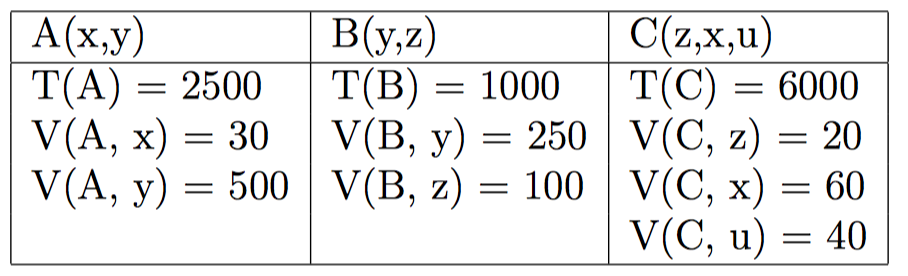
\includegraphics[scale=0.5]{1.png}
	\]
	
	\begin{enumerate}
		\item Draw the B+ tree that would result from inserting a data entry with key 13.\\
		\textbf{Solutions: }
		\[
		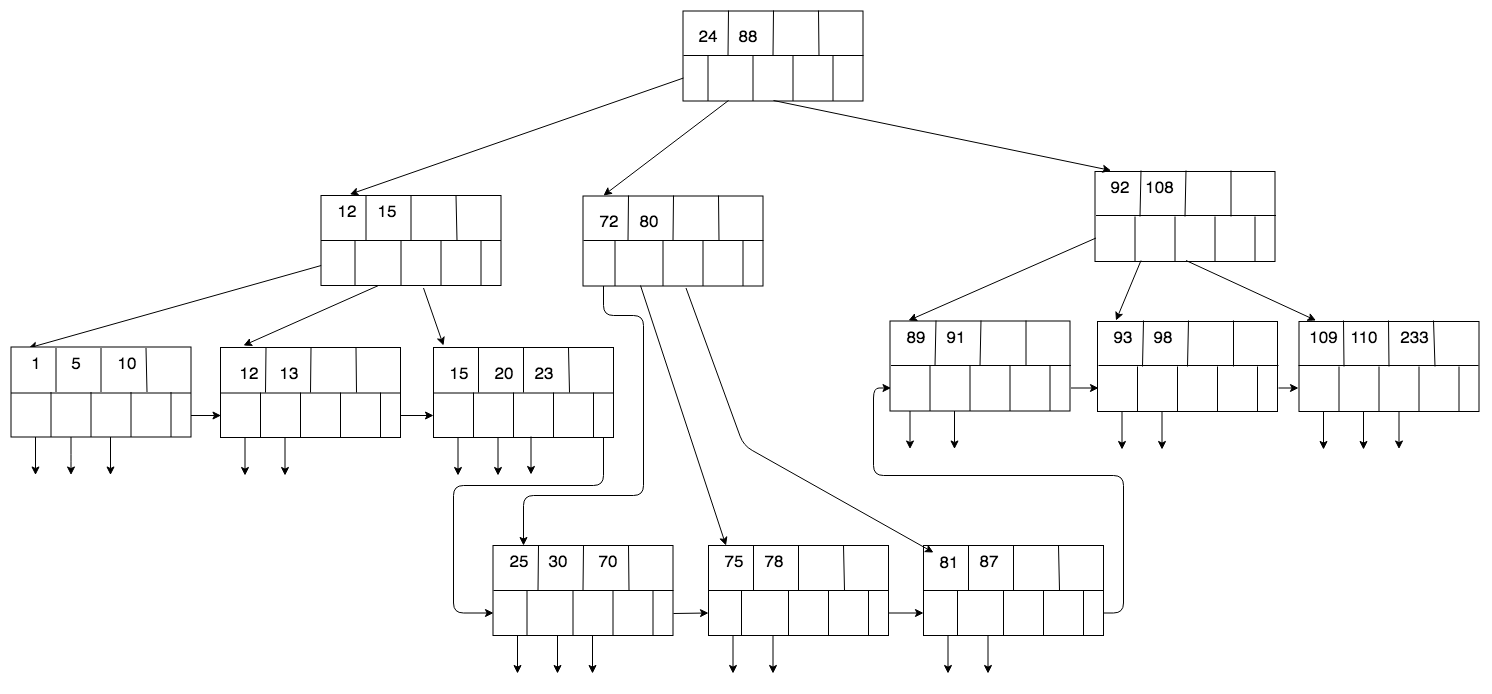
\includegraphics[scale=0.3]{3.png}
		\]
		
		\item Based on the B+ tree that you drew in the previous question, draw the B+ tree that would result from deleting the data entry with key 75.\\
		\textbf{Solutions: }
		\[
		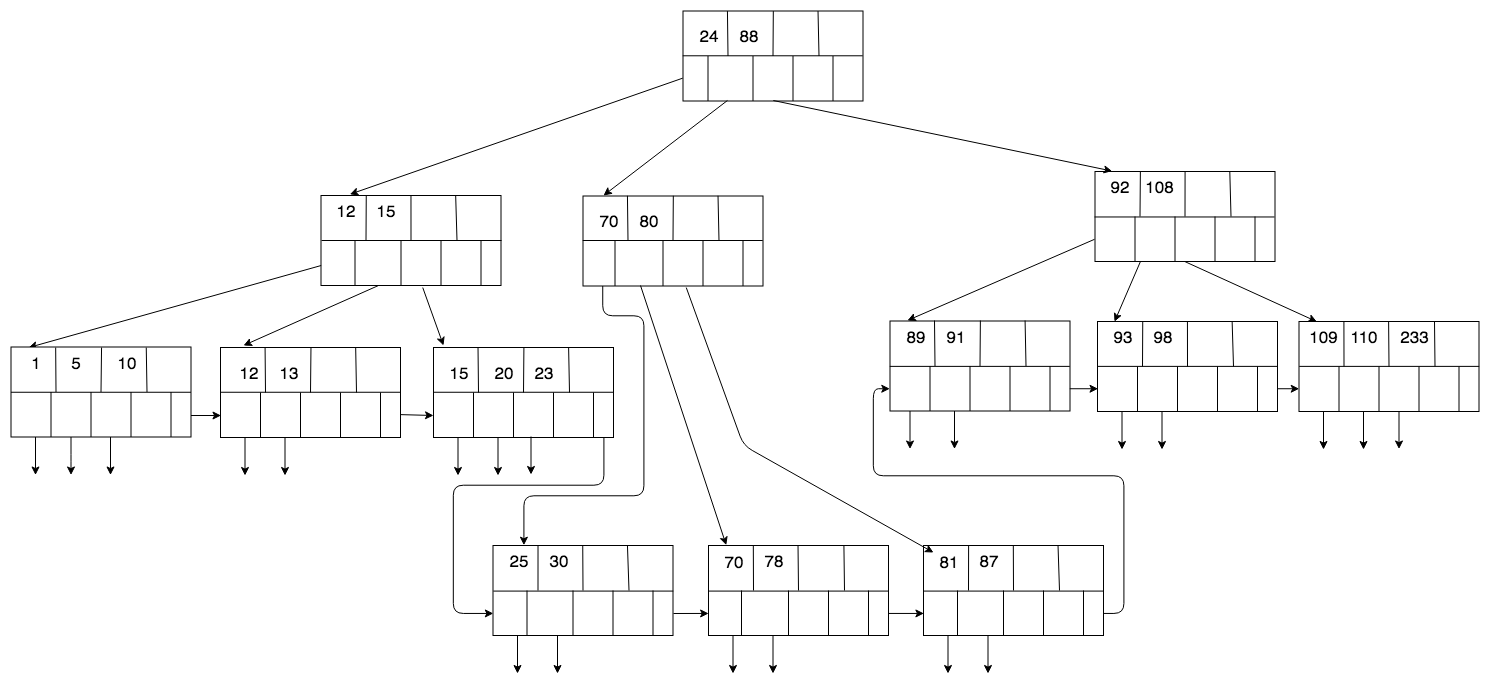
\includegraphics[scale=0.3]{4.png}
		\]
		
		\item Based on the B+ tree that you drew in the previous question, draw the B+ tree that would result from deleting the data entry with key 89.\\
		\textbf{Solutions: }
		\[
		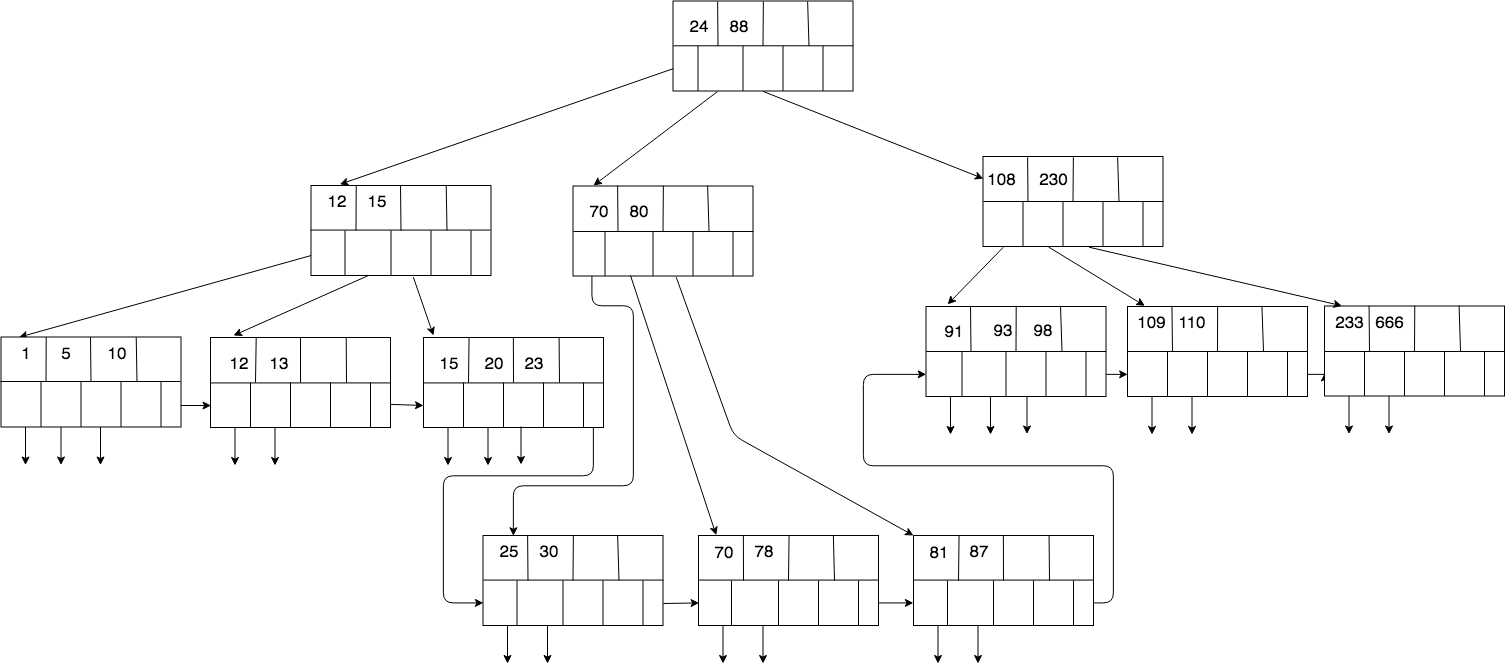
\includegraphics[scale=0.3]{5.png}
		\]
		
	\end{enumerate}
	
	
	\section{Extensible Hashing (30 pts)}
	
	Assume you have a extensible hash table with hash function h(k) = k mod 13, expressed as a binary string of size 4, and data block of size 2 (i.e., it can accommodate two tuples). You are asked to index the following key values in order: 25, 13, 23, 21.
	
	\begin{enumerate}
		\item Draw the extensible hash table which obeys the above constraints after the four keys are inserted.\\
		\textbf{Solutions: }
		First, we apply hash function to every key value.\\
		25 -> 12 -> 1100 \\
		13 -> 0 -> 0000 \\
		23 -> 10 -> 1010 \\
		21 -> 8 -> 1000 \\
		\[
		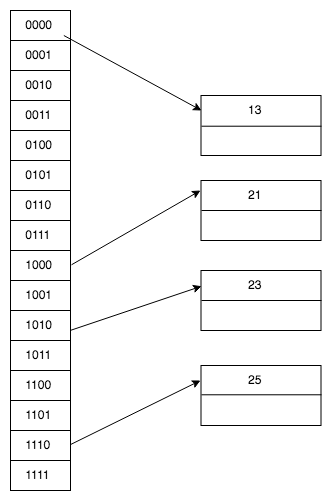
\includegraphics[scale=0.3]{6.png}
		\]
		
		
		\item Using your solution to the previous question, now consider insertion of keys 18 and 20 into the hash table, and draw the resulting hash table.\\
		\textbf{Solutions: }
		First, we apply hash function to every key value.\\
		18 -> 5 -> 0101 \\
		20 -> 7 -> 0111 \\
		\[
		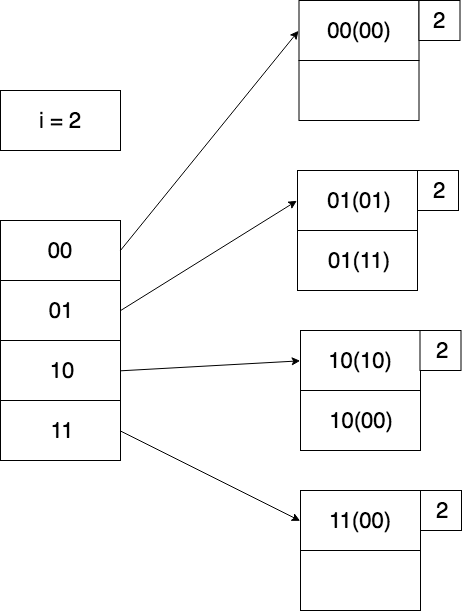
\includegraphics[scale=0.3]{7.png}
		\]
		
	\end{enumerate}
	
	
	
	\section{Linear Hashing (30 pts)}
	
	Consider a linear hash table with $r \leq 1.76n$ with each data block capable of holding 2 records (that is, the average number of record per bucket should not exceed $88\%$ of the total number of records per block):
	
	\[
	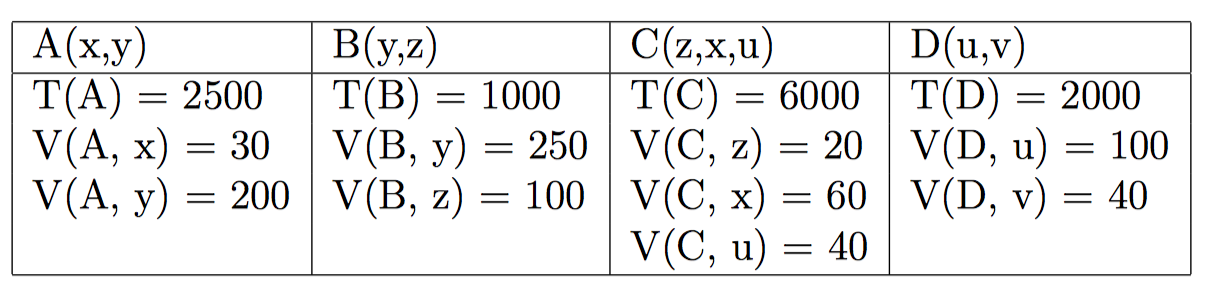
\includegraphics[scale=0.4]{2.png}
	\]
	
	\begin{enumerate}
		\item Insert 1001 and draw the resulting table.\\
		\textbf{Solutions: }
		\[
		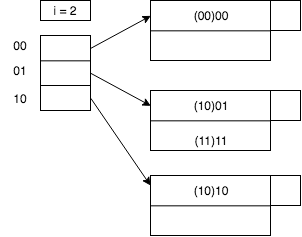
\includegraphics[scale=0.6]{8.png}
		\]
		
		\item With your solution from the previous question, insert 1101, 1110, 0001 incrementally and draw the final table; that is, insert one at a time, check the condition, and move to the next one.\\
		\textbf{Solutions: }
		\[
		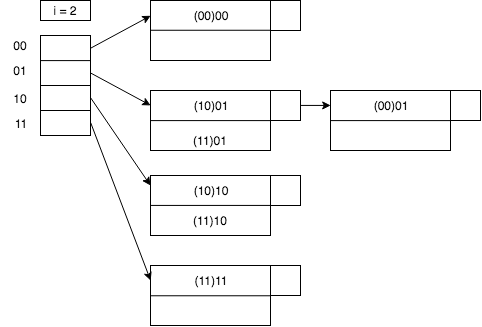
\includegraphics[scale=0.6]{9.png}
		\]
		
	\end{enumerate}
	
	
	
	
	
	%%% End document
\end{document}